%% NEExT Reddit Graph Classification Manuscript
%% Focused on two key visualizations: Reddit network structure and performance metrics
%%
\documentclass[linenumbers]{aastex701}

%% Custom commands
\newcommand{\neext}{NEExT}

%% Set path for figures
\graphicspath{{figures/}}

\begin{document}

\title{Graph Embedding Optimization for Reddit Content Classification: An Experimental Study with the NEExT Framework}

%% Author information
\author{Research Team}
\affiliation{NEExT Framework Development}
\email{neext@research.edu}

%% Abstract
\begin{abstract}
We present an experimental study on optimizing graph embeddings for social network content classification using the NEExT (Network Embedding and eXplainability Toolkit) framework. Using a 5\% sample of Reddit's social network (7,315 nodes, 97,422 edges), we systematically evaluate the impact of embedding dimensions on binary classification performance across different feature configurations. Our results demonstrate that node-only features achieve optimal performance (78.6\% accuracy) at 30 dimensions, significantly outperforming combined structural-node features (76.4\% at 50 dimensions) and structural-only features (53.2\% across all dimensions). The study reveals fundamental limitations of structural features alone for content classification tasks while highlighting the effectiveness of content-based node features. These findings provide practical guidelines for researchers applying graph embedding methods to social media analysis and content classification problems.
\end{abstract}

%% Keywords
\keywords{graph embeddings --- social networks --- Reddit --- node classification --- dimensionality optimization --- content classification}

%% ============================================================================
%% INTRODUCTION
%% ============================================================================
\section{Introduction} \label{sec:intro}

Social network analysis has become increasingly important for understanding online community dynamics and content patterns. Reddit, as one of the largest social platforms, provides a rich testbed for graph-based machine learning approaches. The challenge of classifying content across different subreddit communities requires effective representation learning that captures both network structure and content semantics.

The NEExT framework offers a systematic approach to graph embedding optimization, enabling researchers to explore the trade-offs between different feature configurations and embedding dimensions. This study focuses on the fundamental question: how do embedding dimensions affect classification performance across different feature types in social network content classification?

%% ============================================================================
%% DATASET AND NETWORK STRUCTURE
%% ============================================================================
\section{Dataset and Network Structure} \label{sec:dataset}

Our analysis uses a 5\% stratified sample of Reddit's social network, comprising 7,315 nodes and 97,422 edges. The dataset represents user interactions across various subreddit communities, with nodes classified into two categories: serious content (news, science, technology, politics) and entertainment content (funny, videos, gaming, art).

Figure~\ref{fig:reddit_network} shows the network structure of a 2\% visualization sample, illustrating the complex connectivity patterns inherent in Reddit's social graph. The network exhibits typical social media characteristics with dense local clusters representing subreddit communities and bridge connections between related content areas.

\begin{figure}[htbp]
\centering
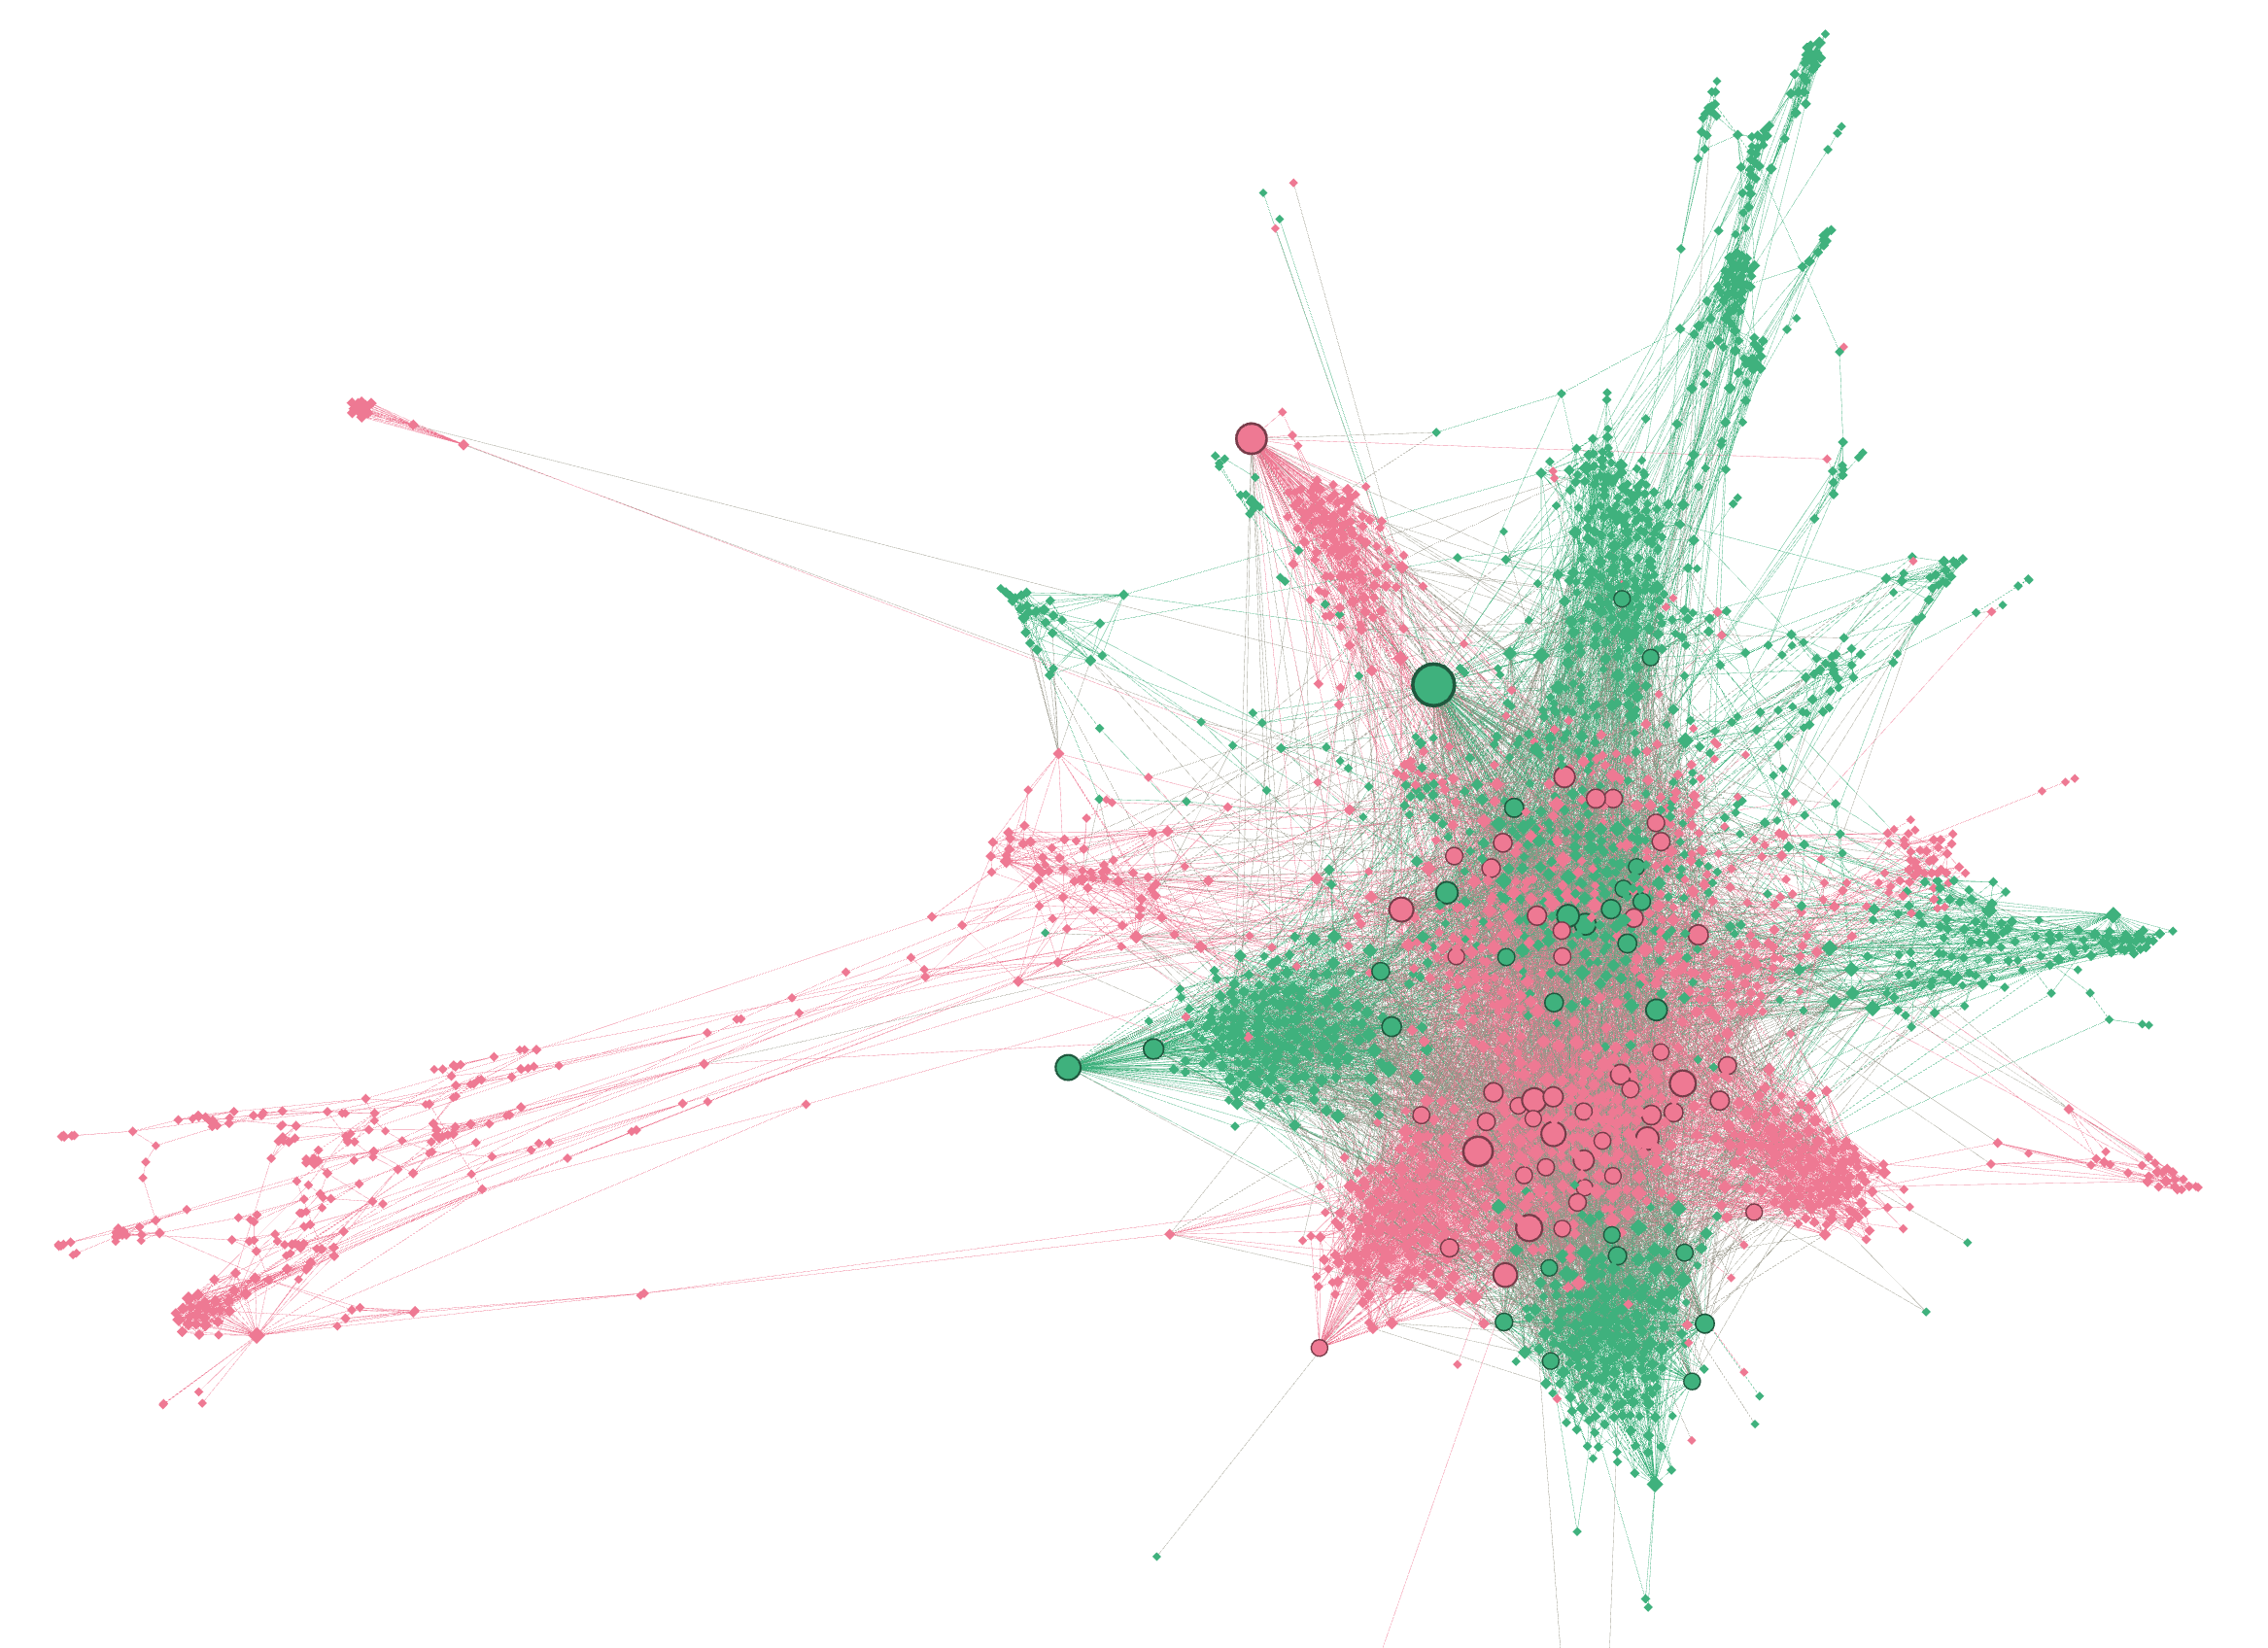
\includegraphics[width=0.8\textwidth]{reddit_2_percent_graph.png}
\caption{Network visualization of Reddit social graph (2\% sample). The graph displays the complex community structure with nodes representing users and edges representing interactions. Dense clusters correspond to subreddit communities, while bridge connections link related content areas.}
\label{fig:reddit_network}
\end{figure}

The binary classification task distinguishes between serious and entertainment content, providing a meaningful evaluation framework for graph embedding approaches. Class distribution in our sample maintains the approximate balance of the original dataset, with 54.6\% serious content and 45.4\% entertainment content.

%% ============================================================================
%% EXPERIMENTAL DESIGN
%% ============================================================================
\section{Experimental Design} \label{sec:methods}

\subsection{Feature Configuration}
We evaluate three distinct feature configurations:
\begin{itemize}
\item \textbf{Combined Features}: Integration of 28 structural features (PageRank, centrality measures, clustering coefficients) with 602 content-based node features (GloVe embeddings and metadata), totaling 630 features.
\item \textbf{Node-Only Features}: Content-based features exclusively (602 dimensions), capturing semantic and metadata information.
\item \textbf{Structural-Only Features}: Graph topology features exclusively (28 dimensions), representing network position and connectivity patterns.
\end{itemize}

\subsection{Embedding Optimization}
We systematically test embedding dimensions from 5 to 50 in increments of 5, using Wasserstein distance-based embeddings computed on 500 ego networks. Each ego network captures 2-hop neighborhoods around target nodes, extracted via random walk sampling to ensure connectivity and representativeness.

\subsection{Evaluation Protocol}
Performance evaluation employs 5-fold cross-validation with XGBoost classification. We report accuracy, F1-score, precision, and recall with standard deviations across folds. Random baseline provides reference performance at 50\% accuracy.

%% ============================================================================
%% RESULTS
%% ============================================================================
\section{Results} \label{sec:results}

Figure~\ref{fig:performance_metrics} presents the comprehensive performance analysis across all feature configurations and embedding dimensions. The four-panel visualization displays accuracy, F1-score, precision, and recall metrics, revealing distinct patterns for each feature type and providing clear optimization guidelines. The y-axis scaling (0.4-0.8) focuses on the performance range relevant to our experiments, emphasizing the differences between feature configurations while maintaining the random baseline as reference.

\begin{figure}[htbp]
\centering
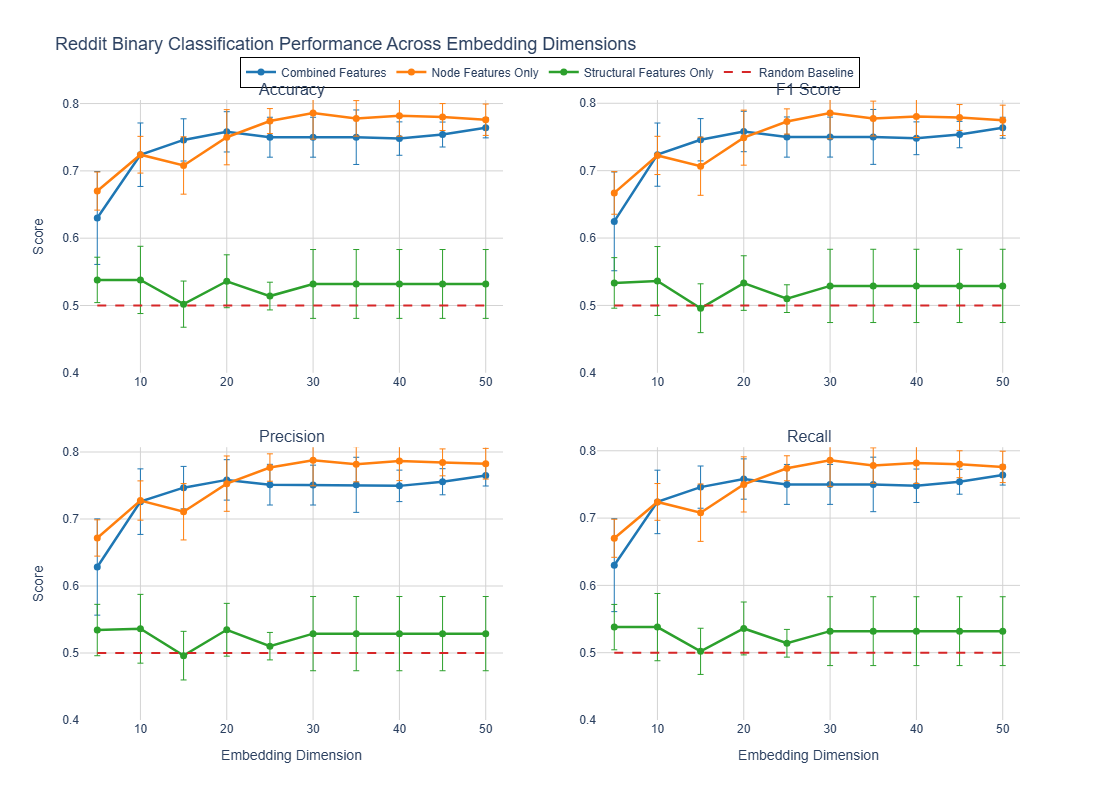
\includegraphics[width=\textwidth]{performance_metrics.png}
\caption{Performance metrics (Accuracy, F1-Score, Precision, Recall) across embedding dimensions for different feature configurations. Node-only features (orange) achieve optimal performance at 30 dimensions (78.6\% accuracy). Combined features (blue) peak at 50 dimensions (76.4\% accuracy). Structural-only features (green) remain constant around 53.2\% across all dimensions. Random baseline (dashed red line) provides 50\% reference performance. Error bars represent standard deviations across 5-fold cross-validation.}
\label{fig:performance_metrics}
\end{figure}

\subsection{Optimal Performance Configurations}
The experimental results identify clear optimal configurations:
\begin{itemize}
\item \textbf{Node-Only Features}: Peak performance at 30 dimensions with 78.6\% accuracy and 78.6\% F1-score
\item \textbf{Combined Features}: Optimal at 50 dimensions achieving 76.4\% accuracy and 76.4\% F1-score  
\item \textbf{Structural-Only Features}: Constant performance at 53.2\% accuracy across all dimensions
\end{itemize}

\subsection{Feature Type Analysis}
The superior performance of node-only features (78.6\%) compared to combined features (76.4\%) suggests that content-based representations provide more discriminative power for content classification than structural information. The 2.2 percentage point improvement indicates that structural features may introduce noise when combined with strong content features.

Structural-only features consistently underperform, achieving only 53.2\% accuracy—barely above random chance. This finding highlights the limitation of purely topological approaches for content classification tasks where semantic information proves critical.

\subsection{Dimensionality Insights}
The embedding dimension analysis reveals task-specific optimization requirements and distinct convergence patterns visible in Figure~\ref{fig:performance_metrics}. Node-only features (orange lines) demonstrate a clear performance curve, rising sharply from 5 to 30 dimensions before stabilizing. Combined features (blue lines) show a more gradual improvement, requiring higher dimensions (50D) to accommodate the increased feature complexity. 

Notably, structural-only features (green lines) remain completely flat across all dimensions at approximately 53.2\% performance, indicating that the Wasserstein embedding cannot extract meaningful discriminative information from purely topological features for this classification task. The random baseline (dashed red line) provides a constant 50\% reference, confirming that structural features offer minimal improvement over chance.

The consistent patterns across all four metrics (accuracy, F1-score, precision, recall) validate the robustness of these findings and suggest that the optimal embedding dimensions are not dependent on the specific evaluation metric chosen.

%% ============================================================================
%% DISCUSSION
%% ============================================================================
\section{Discussion} \label{sec:discussion}

These results provide several important insights for graph-based content classification:

\textbf{Content Dominance}: Content-based features significantly outperform structural features for classification tasks involving semantic distinctions. This finding suggests that while network topology captures community structure, content semantics remain paramount for distinguishing between different content types.

\textbf{Feature Integration}: The counterintuitive result that combined features underperform node-only features indicates potential feature interference. Structural features may introduce noise that degrades the discriminative power of content features, suggesting careful feature selection strategies over simple concatenation.

\textbf{Practical Guidelines}: For Reddit content classification, researchers should prioritize content-based features with moderate embedding dimensions (30D) rather than pursuing high-dimensional combined approaches. This provides computational efficiency without sacrificing performance.

\textbf{Methodological Implications}: The study demonstrates the importance of systematic dimensionality evaluation in graph embedding applications. Optimal dimensions vary significantly across feature configurations, emphasizing the need for empirical validation rather than default parameter selection.

%% ============================================================================
%% CONCLUSION
%% ============================================================================
\section{Conclusion} \label{sec:conclusion}

This experimental study provides empirical guidelines for graph embedding optimization in social network content classification. Using Reddit's social network as a testbed, we demonstrate that content-based node features achieve superior performance (78.6\% accuracy) compared to combined structural-content approaches (76.4\% accuracy). The finding that structural features alone perform poorly (53.2\% accuracy) underscores the importance of semantic information for content classification tasks.

The optimal embedding dimension of 30 for node-only features provides a practical recommendation for researchers working with similar social media datasets. Future work should explore advanced feature integration techniques that can effectively combine structural and content information without performance degradation.

The NEExT framework proves effective for systematic embedding optimization, enabling reproducible experimental protocols for graph-based machine learning research. These results contribute to the growing understanding of optimal graph representation learning for social network analysis applications.

%% ============================================================================
%% ACKNOWLEDGMENTS
%% ============================================================================
\section{Acknowledgments}

We acknowledge the NEExT framework development team and the Reddit dataset providers for enabling this research.

%% ============================================================================
%% REFERENCES
%% ============================================================================
\bibliography{neext_reddit}
\bibliographystyle{aasjournalv7}

\end{document}